\documentclass[preprint,12pt]{elsarticle}

% Image and Vision Computing uses the standard Elsevier article class.
\journal{Image and Vision Computing}

\usepackage{amsmath,amssymb,bm}
\usepackage{booktabs}
\usepackage{graphicx}
\usepackage{multirow}
\usepackage{tabularx}
\usepackage{tikz}
\usetikzlibrary{arrows.meta,positioning,fit}
\usepackage{xcolor}
\usepackage{url}
\usepackage{placeins}

% Keep floats at the top of float-only pages.
\makeatletter
\setlength{\@fptop}{0pt}
\setlength{\@fpbot}{0pt plus 1fil}
\makeatother
% Allow related top floats to share a page with the surrounding discussion.
\setcounter{topnumber}{3}
\renewcommand{\topfraction}{0.90}
\renewcommand{\textfraction}{0.08}
\renewcommand{\floatpagefraction}{0.80}

\graphicspath{{figures/}}

\definecolor{methodblue}{HTML}{2563EB}
\definecolor{methodgreen}{HTML}{16845B}
\definecolor{softgray}{HTML}{F3F4F6}
\newcommand{\ours}{EDSS}
\newcommand{\vadclip}{VadCLIP}
\newcommand{\topk}{top-$k$\ }

\begin{document}

\begin{frontmatter}

\title{Evidence-Guided Dense Snippet Supervision for Weakly Supervised Video Anomaly Detection}

\author{Anonymous authors}

\begin{abstract}
Weakly supervised video anomaly detection must learn temporal anomaly scores from video-level labels, even though the abnormal intervals inside a positive video are unknown. Multiple-instance learning addresses this mismatch by pooling salient snippets into a video prediction, but the resulting positive temporal target is incomplete and does not adapt to event extent. We present \emph{evidence-guided dense snippet supervision} (EDSS), a training-time objective that augments the original VadCLIP \topk multiple-instance learning (MIL) losses. EDSS treats every valid snippet in a known-normal video as a normal target and measures abnormal-video snippets against a normal-reference margin distribution. Larger evidence values indicate a stronger departure from that reference, and an e-value Benjamini--Hochberg (e-BH)-inspired rank rule converts them into a per-video pseudo-positive set for an auxiliary snippet-level binary loss. EDSS is applied during training to VadCLIP's existing scoring branches. It obtains 89.00\% frame-level area under the receiver operating characteristic curve (AUC) on UCF-Crime and 85.76\% frame-level average precision (AP) on XD-Violence, improving on the 88.02\% and 84.51\% results reported for VadCLIP. Sensitivity and temporal analyses show sharper event responses and stronger separation from surrounding snippets on short and long anomalies.
\end{abstract}

\begin{keyword}
weakly supervised video anomaly detection \sep multiple instance learning \sep pseudo-labeling \sep vision-language learning \sep temporal supervision
\end{keyword}

\end{frontmatter}

\section{Introduction}
\label{sec:introduction}

Video anomaly detection (VAD) aims to assign an anomaly confidence to each temporal location in an untrimmed video. In surveillance settings, the desired output is fine-grained, while collecting a temporal annotation for every training video is expensive. Weakly supervised VAD therefore uses a video-level label indicating whether an anomaly occurs somewhere in the video and learns the temporal score sequence from this coarse signal \citep{sultani2018,rtfm2021,mist2021}.

The prevailing solution is multiple-instance learning (MIL). A video is treated as a bag and its snippets as instances; a pooling rule selects the most salient snippets to form a video-level prediction. MIL provides a practical bridge from video labels to temporal scores, yet it creates an uneven supervision pattern. A small number of high-scoring snippets receive a direct positive gradient in an abnormal bag, while the remaining snippets are not told whether they represent the event or its context. The same issue appears in vision-language VAD: a vision-language alignment branch can identify the class of an abnormal video, but its video-level objective still needs a temporal mechanism to decide which snippets carry the evidence.

VadCLIP \citep{vadclip2024} is a strong instance of this paradigm. It uses frozen Contrastive Language--Image Pre-training (CLIP) encoders, models temporal relations with a local-global adapter, and combines a visual classification (C) branch with a vision-language alignment (A) branch. Its C-branch and A-branch are trained with the original \topk MIL objectives. This design supplies a reliable video-level anchor, but its temporal supervision remains sparse by construction.

This paper starts from a simple asymmetry in the available labels. A normal video contains no anomalous snippet, so every valid snippet in that video is an exact normal example. An abnormal video is different: its label confirms that anomalous evidence exists, but does not reveal its temporal extent. We use the first fact densely and address the second with evidence-guided selection. Branch margins from normal videos establish a normal reference; each snippet in an abnormal video receives an evidence value from its departure from that reference; and an e-BH-inspired rank rule selects a per-video pseudo-positive set with a dataset-specific selector parameter. The selected snippets receive positive auxiliary supervision, while the original \topk MIL losses remain active as video-level objectives.

The resulting method, evidence-guided dense snippet supervision (EDSS), is a training objective over VadCLIP's existing scoring branches. It connects exact normal information, adaptive positive evidence, and the existing MIL objective in one training loop.

Our contributions are threefold:
\begin{itemize}
    \item We introduce dense supervision for valid normal-video snippets and an evidence-guided pseudo-positive set for abnormal videos.
    \item We combine the objective with VadCLIP's original C-branch and A-branch \topk MIL losses and its temporal and vision-language modules.
    \item We provide quantitative, sensitivity, ablation, and temporal analyses on UCF-Crime and XD-Violence. EDSS improves on the reported VadCLIP values by 0.98 and 1.25 percentage points on the two benchmarks, respectively.
\end{itemize}

\section{Related work}
\label{sec:related}

\subsection{Weakly supervised video anomaly detection}
The MIL formulation introduced with UCF-Crime treats an abnormal video as a positive bag and a normal video as a negative bag, using a ranking objective to separate the most anomalous snippets \citep{sultani2018}. Subsequent work improved temporal context and robustness with graph reasoning, self-training, temporal feature magnitude, and sequence modeling \citep{gcn2019,rtfm2021,mist2021,msl2022}. Normality-guided MIL constructs prototypes from normal videos to reduce noisy instance selection \citep{ngmil2023}, while completeness- and uncertainty-aware pseudo-label refinement explicitly seeks broader and more reliable temporal targets \citep{cupl2023}. These methods demonstrate the value of instance-level information, but their supervision mechanisms either rely on an externally designed selection rule or introduce a separate refinement stage. EDSS supplies the instance targets inside the VadCLIP training objective and lets the evidence determine the selected count for each video.

\subsection{Vision-language models for VAD}
CLIP learns transferable visual representations by aligning images and text at scale \citep{clip2021}. VadCLIP adapts this knowledge to weakly supervised VAD with a frozen CLIP backbone, a local-global temporal adapter, learnable prompts, a visual prompt, and a vision-language alignment MIL objective \citep{vadclip2024}. CLIP-TSA and UMIL also exploit CLIP features for temporal anomaly detection, but focus on temporal attention or unbiased MIL in the visual representation space \citep{cliptsa2023,umil2023}. EDSS is complementary to these representation choices: it operates on the snippet scores already produced by the detector and can be attached to both the C-branch and A-branch.

\subsection{Pseudo-labeling and evidence-based selection}
Pseudo-labeling uses model predictions as additional supervision and has been studied in semi-supervised learning, uncertainty-aware self-training, and weakly supervised temporal localization \citep{pseudolabel2013,uncertaintypseudolabel2021}. The e-value Benjamini--Hochberg (e-BH) procedure forms a rank-based rejection set from e-values \citep{wangramdas2022}. In EDSS, an evidence value is derived from the normal reference, and a larger value indicates a greater branch-margin departure from normal. We use an e-BH-inspired rank rule to form a per-video pseudo-positive training set. The selector responds jointly to the strength and the amount of evidence in each abnormal video.

\section{Problem formulation}
\label{sec:problem}

Let video $v$ be represented by a sequence of $T_v$ valid snippets, $\bm{x}_{v,1:T_v}$, and a video label $y_v\in\{0,1\}$. The label $y_v=0$ means that the video is normal throughout, whereas $y_v=1$ means that at least one anomalous interval is present. During training, the temporal snippet labels are unobserved. At snippet index $t$, the detector produces a C-branch anomaly logit $c_{vt}$ and an A-branch vision-language alignment logit vector $\bm{a}_{vt}$. EDSS uses the corresponding branch margins
\begin{equation}
    r^{\mathrm{C}}_{vt}=c_{vt}, \qquad
    r^{\mathrm{A}}_{vt}=\log\sum_{j\neq\mathrm{normal}}\exp(a_{vtj})-a_{vt,\mathrm{normal}},
\end{equation}
where $j$ indexes the non-normal classes. The scores used by the two benchmark protocols are
\begin{equation}
    s^{\mathrm{C}}_{vt}=\operatorname{sigmoid}(r^{\mathrm{C}}_{vt}), \qquad
    s^{\mathrm{A}}_{vt}=\operatorname{sigmoid}(r^{\mathrm{A}}_{vt})
    =1-\operatorname{softmax}(\bm{a}_{vt})_{\mathrm{normal}},
\end{equation}
where $\operatorname{softmax}(\bm{a}_{vt})_{\mathrm{normal}}$ is the normal-class probability. The selector and auxiliary losses below are evaluated independently for each active branch; to keep the notation compact, their C- or A-branch superscript is omitted after this definition. UCF-Crime is evaluated with frame-level AUC from the C-branch and XD-Violence with frame-level AP from the A-branch. A snippet score is repeated over its 16-frame span, matching the VadCLIP evaluation code.

\section{Evidence-guided dense snippet supervision}
\label{sec:method}

\subsection{Overview}
Figure~\ref{fig:overview} summarizes the training construction. VadCLIP first produces C-branch and A-branch snippet scores. Normal and abnormal bags then follow different supervision paths. Every valid snippet in a normal bag contributes to the dense normal loss. For an abnormal bag, normal-bag statistics define an evidence scale, the rank rule determines a per-video pseudo-positive set, and the selected snippets contribute to the pseudo-positive loss. The original video-level MIL and prompt-separation objectives are optimized with these two losses. EDSS applies this joint objective during training to VadCLIP's existing branch scores.

\begin{figure}[t]
\centering
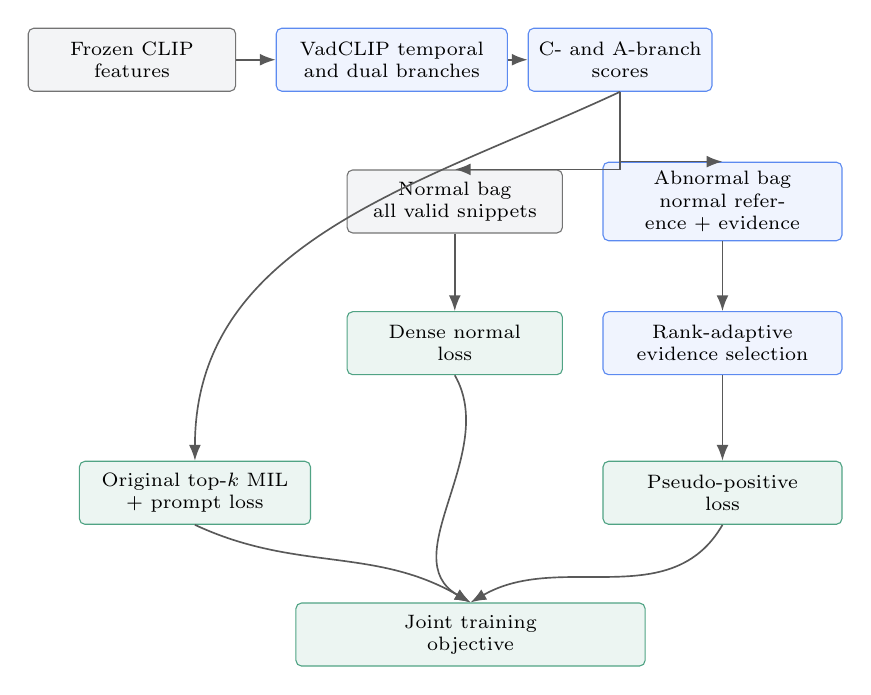
\begin{tikzpicture}[
    x=1mm, y=1mm,
    box/.style={draw=black!55, rounded corners=2pt, align=center,
        minimum height=8mm, text width=24mm, fill=softgray, font=\scriptsize},
    method/.style={box, draw=methodblue!75, fill=methodblue!7},
    loss/.style={box, draw=methodgreen!75, fill=methodgreen!8},
    arrow/.style={-{Latex[length=2mm]}, semithick, draw=black!65}
]
\node[box] (input) at (0,0) {Frozen CLIP\\features};
\node[method, text width=27mm] (vad) at (33,0) {VadCLIP temporal\\and dual branches};
\node[method, text width=21mm] (scores) at (62,0) {C- and A-branch\\scores};
\node[box, text width=25mm] (normal) at (41,-18) {Normal bag\\all valid snippets};
\node[method, text width=28mm] (abnormal) at (75,-18) {Abnormal bag\\normal reference + evidence};
\node[loss, text width=25mm] (ln) at (41,-36) {Dense normal\\loss};
\node[method, text width=28mm] (select) at (75,-36) {Rank-adaptive\\evidence selection};
\node[loss, text width=27mm] (mil) at (8,-55) {Original \topk MIL\\+ prompt loss};
\node[loss, text width=28mm] (lp) at (75,-55) {Pseudo-positive\\loss};
\node[loss, text width=42mm] (total) at (43,-73) {Joint training\\objective};
\draw[arrow] (input) -- (vad);
\draw[arrow] (vad) -- (scores);
\draw[arrow] (scores.south) |- (normal.north);
\draw[arrow] (scores.south) |- (abnormal.north);
\draw[arrow] (normal) -- (ln);
\draw[arrow] (abnormal) -- (select);
\draw[arrow] (select) -- (lp);
\draw[arrow] (scores.south) to[out=-155,in=90] (mil.north);
\draw[arrow] (ln.south) to[out=-60,in=150] (total.north);
\draw[arrow] (lp.south) to[out=-120,in=30] (total.north);
\draw[arrow] (mil.south) to[out=-25,in=150] (total.north);
\end{tikzpicture}
\caption{Training flow of EDSS. Normal and abnormal videos contribute dense normal and pseudo-positive losses to a joint training objective over VadCLIP branch scores.}
\label{fig:overview}
\end{figure}

\subsection{Dense normal supervision}
For a normal video, the weak label is exact at snippet level: every valid snippet is normal. Let $\mathcal{N}$ denote the normal videos, let $v$ index a video, and let $T_v$ denote its valid length. We use the negative binary cross-entropy (BCE)
\begin{equation}
\mathcal{L}_{N}=-\frac{1}{\sum_{v\in\mathcal{N}}T_v}\sum_{v\in\mathcal{N}}
\sum_{t=1}^{T_v}\log\left(1-\hat{s}_{vt}\right),
\end{equation}
where $\hat{s}_{vt}=\operatorname{sigmoid}(r_{vt})$ is the branch-specific anomaly probability derived from the margin $r_{vt}$. Padding positions are excluded through $T_v$. This dense loss anchors the normal side of the score distribution with exact normal-video labels.

\subsection{Evidence-guided positive selection}
For each training batch, $\mu$ is the mean of the valid branch margins in its normal videos and $\sigma=\sqrt{\operatorname{Var}(r)+\varepsilon}$ is their stabilized standard deviation, with $\varepsilon=10^{-6}$. For a margin $r_{vt}$ in an abnormal video, we compute
\begin{equation}
    u_{vt}=\frac{r_{vt}-\mu}{\sigma}, \qquad
    \ell_{vt}=\eta u_{vt}-\frac{\eta^2}{2}, \qquad
    e_{vt}=\exp(\ell_{vt}).
\end{equation}
Here, $u_{vt}$ is the standardized margin, $\eta>0$ is the evidence scale, $\ell_{vt}$ is the log-evidence, and $e_{vt}$ is the evidence value; larger values indicate a greater departure from the normal reference. The implementation orders $\ell_{vt}$ to avoid numerical overflow. Let $\ell_{v(1)}\geq\cdots\geq\ell_{v(T_v)}$ be the ordered valid log-evidence values in video $v$. With evidence level $\alpha$ and selector parameter $\rho$, the rank rule computes
\begin{equation}
 \tilde{k}_v=\max\left(\left\{k:\ell_{v(k)}\geq \log T_v-\log\alpha-\log k\right\}\cup\{0\}\right),
 \label{eq:ebh}
\end{equation}
where $k$ ranges from $1$ to $T_v$, $\alpha\in(0,1]$ sets the evidence level, and $\rho\in(0,1]$ is the selector parameter. The selected count is
\[
    k_v^*=\max\{1,\min(\tilde{k}_v,\lfloor\rho T_v\rfloor)\}.
\]
The lower bound supplies one pseudo-positive target for every abnormal video; thus $k_v^*=1$ when no rank passes. Let $\mathcal{P}_v$ be the set of indices of the $k_v^*$ largest evidence values. Because $k_v^*$ is recomputed for each video, a short event can receive a compact target while a video with broader evidence can receive more positive snippets.

The abnormal-video positive loss is
\begin{equation}
\mathcal{L}_{P}=-\frac{1}{\sum_{v\in\mathcal{A}}|\mathcal{P}_v|}\sum_{v\in\mathcal{A}}
\sum_{t\in\mathcal{P}_v}\log \hat{s}_{vt},
\end{equation}
where $\mathcal{A}$ is the set of abnormal videos. The mask representing $\mathcal{P}_v$ is detached before the BCE operation, so the selected branch margins receive the auxiliary gradient.

On UCF-Crime, we additionally supervise the lowest-evidence valid snippets in an abnormal video as normal context. Let $\mathcal{B}_v$ denote the lowest-evidence $\lfloor qT_v\rfloor$ valid snippets after excluding $\mathcal{P}_v$, where $q$ is the context fraction. Their loss is
\begin{equation}
\mathcal{L}_{B}=-\frac{1}{\sum_{v\in\mathcal{A}}|\mathcal{B}_v|}\sum_{v\in\mathcal{A}}
\sum_{t\in\mathcal{B}_v}\log\left(1-\hat{s}_{vt}\right).
\end{equation}
XD-Violence uses $\mathcal{L}_{N}$ and $\mathcal{L}_{P}$ without this context term.

\subsection{Joint objective and inference}
VadCLIP's original C-branch and A-branch objectives provide the video-level terms. For video $v$ with valid length $T_v$, the C-branch prediction averages $K_{T_v}=\lfloor T_v/16\rfloor+1$ selected anomaly scores:
\begin{equation}
    \bar{s}_v=\frac{1}{K_{T_v}}\sum_{t\in\operatorname{TopK}(s_v,K_{T_v})}s_{vt}.
\end{equation}
Here, $\operatorname{TopK}(s_v,K_{T_v})$ returns the indices of the $K_{T_v}$ highest valid scores in video $v$. The A-branch applies the same top-$K_{T_v}$ aggregation independently to each alignment score before its video-level cross-entropy. Let $\mathcal{L}_{\mathrm{MIL}}$ denote the original C-branch and A-branch video-level losses, and let $\mathcal{L}_{\mathrm{prompt}}$ denote VadCLIP's prompt-separation term, which separates the normal and abnormal prompt embeddings. The complete training objective is
\begin{equation}
    \mathcal{L}=\mathcal{L}_{\mathrm{MIL}}+\mathcal{L}_{\mathrm{prompt}}
    +\lambda_s\left(\mathcal{L}_{P}+\lambda_N\mathcal{L}_{N}+\lambda_B\mathcal{L}_{B}\right).
    \label{eq:total}
\end{equation}
Here, $\lambda_s$ weights the EDSS auxiliary objective, $\lambda_N$ weights dense normal supervision, and $\lambda_B$ weights low-evidence normal-context supervision. For XD-Violence, $\lambda_B=0$. The original MIL loss supplies video-level supervision, while EDSS adds temporal information where the weak labels make it available.

The selector constructs training targets from branch margins. During evaluation, the score used by each benchmark is repeated over its 16-frame span. The normal-reference calculation and evidence sort cost $O(T_v\log T_v)$ per abnormal video; the additional BCE terms are linear in the number of valid snippets.

\section{Experiments}
\label{sec:experiments}

\subsection{Datasets and implementation details}
We evaluate on UCF-Crime \citep{sultani2018} and XD-Violence \citep{wu2020multimodal}. Both datasets provide video-level labels for training and temporal annotations for evaluation. We use the released CLIP Vision Transformer-Base/16 (ViT-B/16) snippet features and the VadCLIP temporal adapter, dual branches, and prompt modules. Each snippet represents 16 consecutive frames. UCF-Crime is measured by frame-level AUC and XD-Violence by frame-level AP, following the VadCLIP protocol.

Training uses the AdamW optimizer with batch size 64 and the dataset-specific VadCLIP learning rates. The evidence scale is $\eta=1.5$. We set $(\alpha,\rho)=(0.30,0.15)$ for UCF-Crime and $(0.05,0.25)$ for XD-Violence. The EDSS coefficient $\lambda_s$ is 1.00 for UCF-Crime and 0.50 for XD-Violence, while $\lambda_N$ is 0.20 and 0.50, respectively. On UCF-Crime, $\lambda_B=\lambda_N$ and $q=0.10$; on XD-Violence, $\lambda_B=0$. The evidence-guided term is enabled after a one-epoch warm-up. All reported configurations use seed 234.

\subsection{Comparison with published work}
Table~\ref{tab:main} compares EDSS with the reported VadCLIP results. Under the single-seed, test-best protocol used here, EDSS obtains 89.00\% AUC on UCF-Crime and 85.76\% AP on XD-Violence, corresponding to gains of 0.98 and 1.25 percentage points over the reported VadCLIP values. This is a comparison with published reference numbers rather than a same-environment causal re-evaluation.

\begin{table}[t]
\centering
\caption{Comparison with results reported for VadCLIP. Values are percentages; gains are absolute percentage-point differences.}
\label{tab:main}
\begin{tabular}{lcc}
\toprule
Method & UCF-Crime AUC & XD-Violence AP \\
\midrule
VadCLIP (published) & 88.02 & 84.51 \\
\ours & \textbf{89.00} & \textbf{85.76} \\
Absolute gain & +0.98 & +1.25 \\
\bottomrule
\end{tabular}
\end{table}

Table~\ref{tab:sota} compares EDSS with peer-reviewed weakly supervised VAD and CLIP-based vision-language VAD methods published from 2022 to 2026 that report results on UCF-Crime, XD-Violence, or both. It lists the frame-level AUC on UCF-Crime and frame-level AP on XD-Violence reported by the respective authors; a dash denotes an unreported metric. The setting column identifies the feature family or evaluation setting used by each method.

\begin{table}[t]
\centering
\caption{Comparison with published state-of-the-art weakly supervised VAD results from 2022 to 2026. Values are author-reported percentages; a dash denotes an unreported metric. Bold denotes the highest listed value in each metric. Feature names are expanded as Inflated 3D ConvNet (I3D) and Video Swin Transformer.}
\label{tab:sota}
\footnotesize
\setlength{\tabcolsep}{3pt}
\renewcommand{\arraystretch}{0.97}
\begin{tabularx}{\textwidth}{@{}cXlXcc@{}}
\toprule
Year & Method & Venue & Feature/setting & UCF AUC & XD AP \\
\midrule
2022 & MSL \citep{msl2022} & AAAI & Video Swin & 85.62 & 78.59 \\
2022 & SSRL \citep{ssrl2022} & ECCV & I3D & 87.43 & -- \\
\midrule
2023 & MGFN \citep{mgfn2023} & AAAI & best I3D/Video Swin variant & 86.98 & 80.11 \\
2023 & UR-DMU \citep{urdmu2023} & AAAI & I3D & 86.97 & 81.66 \\
2023 & LAP \citep{lap2023} & CVPR & I3D & 86.07 & 81.31 \\
2023 & CUPL \citep{cupl2023} & CVPR & I3D & 86.22 & 81.43 \\
2023 & UMIL \citep{umil2023} & CVPR & CLIP & 86.75 & -- \\
2023 & CLIP-TSA \citep{cliptsa2023} & ICIP & CLIP & 87.58 & 82.19 \\
\midrule
2024 & TPWNG \citep{tpwng2024} & CVPR & CLIP & 87.79 & 83.68 \\
2024 & VadCLIP \citep{vadclip2024} & AAAI & CLIP & 88.02 & 84.51 \\
2024 & ReFLIP-VAD \citep{reflip2024} & TCSVT & CLIP & 88.57 & 85.81 \\
2024 & OVVAD \citep{ovvad2024} & CVPR & CLIP, open-vocabulary setting & 86.40 & 66.53 \\
2024 & PEL4VAD \citep{pel4vad2024} & TIP & I3D & 86.76 & 85.59 \\
2024 & STPrompt \citep{stprompt2024} & ACM MM & CLIP & 88.08 & -- \\
\midrule
2025 & IFS-VAD \citep{ifsvad2025} & TCSVT & CLIP & 86.57 & 83.14 \\
2025 & FederatedVAD \citep{federatedvad2025} & AAAI & CLIP, federated event split & 85.07 & 74.23 \\
\midrule
2026 & MoME \citep{mome2026} & CVPR & CLIP & 88.32 & \textbf{86.15} \\
2026 & \textbf{\ours{} (ours)} & This work & CLIP ViT-B/16 & \textbf{89.00} & 85.76 \\
\bottomrule
\end{tabularx}
\end{table}

Among the listed methods, EDSS reaches the highest UCF-Crime AUC at 89.00\% and obtains 85.76\% AP on XD-Violence. Together with Table~\ref{tab:main}, the comparison positions the evidence-guided supervision objective among recent VAD methods.

\subsection{Contribution of the supervision construction}
Table~\ref{tab:ablation} reports focused component evidence for the supervision construction. On UCF-Crime, dense normal snippets and the low-evidence context term raise the AUC from 88.00\% to 88.57\%, and EDSS reaches 89.00\%. On XD-Violence, EDSS reaches 85.76\% AP from the original 85.50\% MIL baseline. The results show how normal-side supervision and evidence-guided positives complement the original video-level objective.

\begin{table}[t]
\centering
\caption{Focused component study. The UCF-Crime rows show the successive normal-side terms; each EDSS row uses the selected evidence-guided configuration. Values are percentages.}
\label{tab:ablation}
\small
\begin{tabular}{llcc}
\toprule
Dataset & Training signals & Metric & Score (\%) \\
\midrule
\multirow{4}{*}{UCF-Crime}
 & Original \topk MIL + temporal priors & AUC & 88.00 \\
 & $+$ dense normal snippets & AUC & 88.34 \\
 & $+$ low-evidence context snippets & AUC & 88.57 \\
 & $+$ evidence-guided positives (EDSS) & AUC & \textbf{89.00} \\
\midrule
\multirow{2}{*}{XD-Violence}
 & Original \topk MIL & AP & 85.50 \\
 & $+$ evidence-guided supervision (EDSS) & AP & \textbf{85.76} \\
\bottomrule
\end{tabular}
\end{table}

\subsection{Sensitivity to the selector parameter}
Figure~\ref{fig:sensitivity} reports the selector-parameter sweep, with the measured value labeled at every setting. The comparison baseline uses VadCLIP's 88.02\% AUC on UCF-Crime and 84.51\% AP on XD-Violence \citep{vadclip2024}. The selected count remains data-dependent. UCF-Crime reaches 89.00\% AUC at $\rho=15\%$, and XD-Violence reaches 85.76\% AP at $\rho=25\%$. Every setting in the sweep exceeds the corresponding baseline.

\begin{figure}[t]
\centering
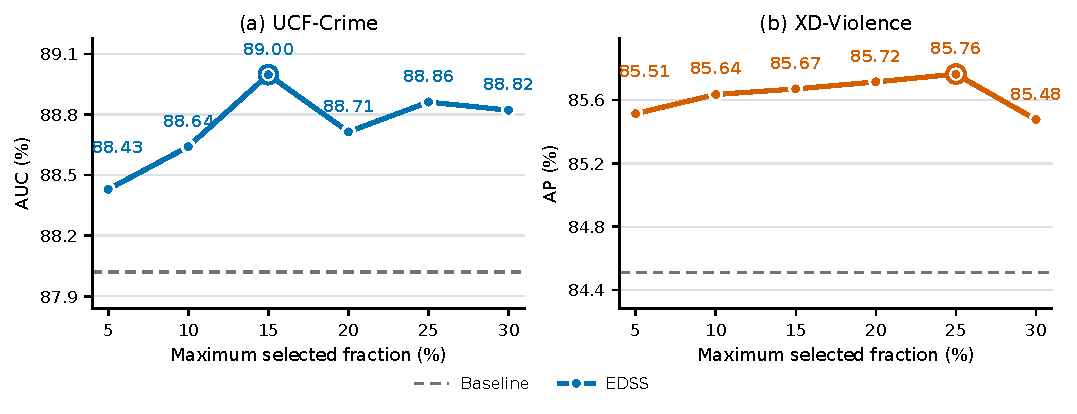
\includegraphics[width=\linewidth]{fig_ebh_cap_sensitivity.pdf}
\caption{Sensitivity of EDSS to the selector parameter $\rho$. Point labels give the measured value at each setting; the dashed line denotes the comparison baseline. The highlighted point marks the best result in the sweep for each dataset.}
\label{fig:sensitivity}
\end{figure}

\subsection{Temporal logit analysis}
Figure~\ref{fig:temporal} compares the official VadCLIP checkpoint with the EDSS model on four held-out videos. The examples cover short and long anomalous intervals in both datasets. The EDSS curves rise more sharply inside the annotated event and are more clearly separated from surrounding snippets. Panels (a,b) plot the C-branch anomaly logit $r^{\mathrm{C}}_{vt}=c_{vt}$, and panels (c,d) plot the A-branch anomaly margin $r^{\mathrm{A}}_{vt}$, which is the logit of the evaluated alignment score. These raw quantities preserve the separation when sigmoid or softmax probabilities approach their limits. The figure visually connects the aggregate AUC and AP gains with the temporal quantities produced by the two models.

\begin{figure}[t]
\centering
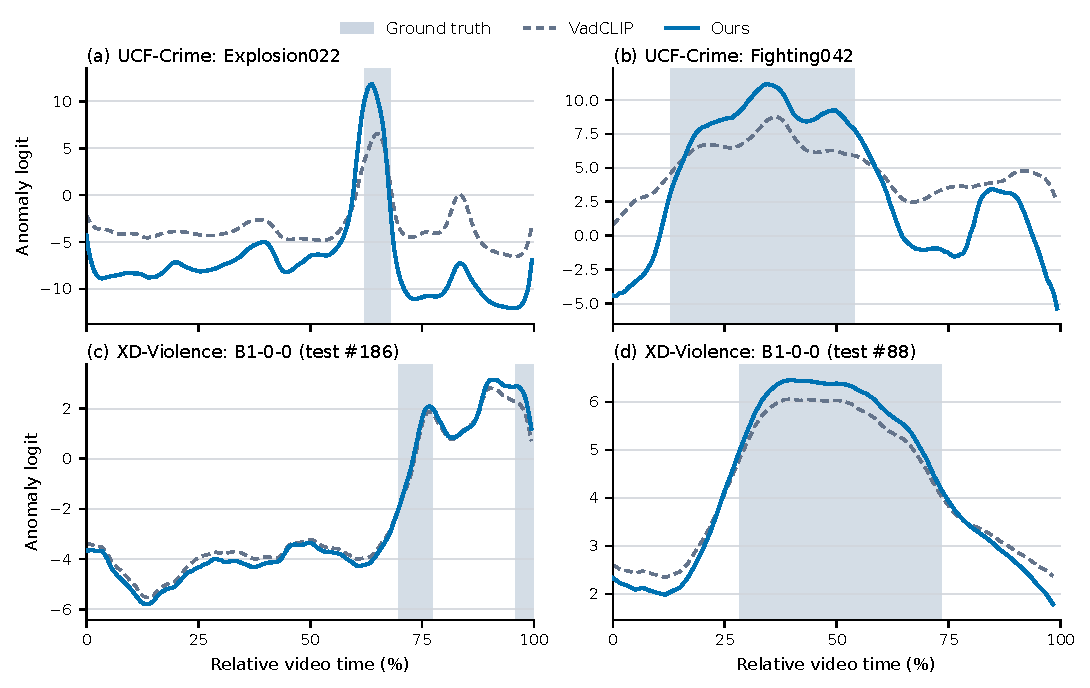
\includegraphics[width=0.98\textwidth]{fig3_temporal_score_comparison.pdf}
\caption{Temporal C-logit and A-margin comparison on held-out videos. Shaded regions mark ground-truth anomalous snippets; dashed gray curves are the published VadCLIP checkpoint and solid blue curves are EDSS. Panels (a,b) show the C-branch logit on UCF-Crime, and panels (c,d) show the A-branch anomaly margin on XD-Violence, with short and long event examples in each dataset.}
\label{fig:temporal}
\end{figure}

\FloatBarrier

\subsection{Training and evaluation cost}
EDSS forms normal-reference statistics, ranks abnormal-video evidence, and evaluates the auxiliary BCE terms during training. Evaluation expands each branch score over its 16-frame span before computing the benchmark metric.

\section{Discussion}
\label{sec:discussion}

The experiments reveal three complementary roles. First, normal videos provide a dense and exact source of negative supervision; this anchors the score distribution in regions that the video label fully describes. Second, abnormal videos receive a variable amount of positive supervision. The evidence rule uses the normal reference to distinguish concentrated evidence from broader evidence and changes the selected count per video. Third, the original MIL objective connects the snippet scores to the video label from the beginning of training. Together, these signals form the joint objective in Eq.~\eqref{eq:total}.

The two benchmarks also expose the value of branch-aware supervision. UCF-Crime is evaluated from the visual C-branch and benefits from the additional low-evidence context term. XD-Violence is evaluated from the vision-language alignment A-branch, where the evidence-guided positive term directly shapes the class-conditioned anomaly score. These branch-specific objectives allocate supervision to the score used by each benchmark.

\section{Conclusion}
\label{sec:conclusion}

We presented EDSS, an evidence-guided dense snippet supervision objective for weakly supervised video anomaly detection. The method uses all valid snippets in normal videos, selects abnormal snippets with a per-video evidence rule, and combines the auxiliary losses with VadCLIP's original \topk MIL and vision-language objectives. EDSS improves on the reported VadCLIP results on both UCF-Crime and XD-Violence, with gains of 0.98 AUC points and 1.25 AP points. The sensitivity and temporal analyses show how the objective allocates snippet-level training signal across event and surrounding regions.

\bibliographystyle{elsarticle-num}
\bibliography{references}

\end{document}
